\chapter{Datos AEMET}
\label{appendix:datos_aemet}

\section{Obtención de datos}

Para descargar los datos de las ciudades ha sido necesario obtener una API key para acceder al sistema de Open Data (\url{https://opendata.aemet.es/centrodedescargas/inicio}, ver figura \ref{fig:panel_aemet}).

\begin{figure}[h]
  \caption{Panel de descarga de datos de AEMET}
  \label{fig:panel_aemet}
  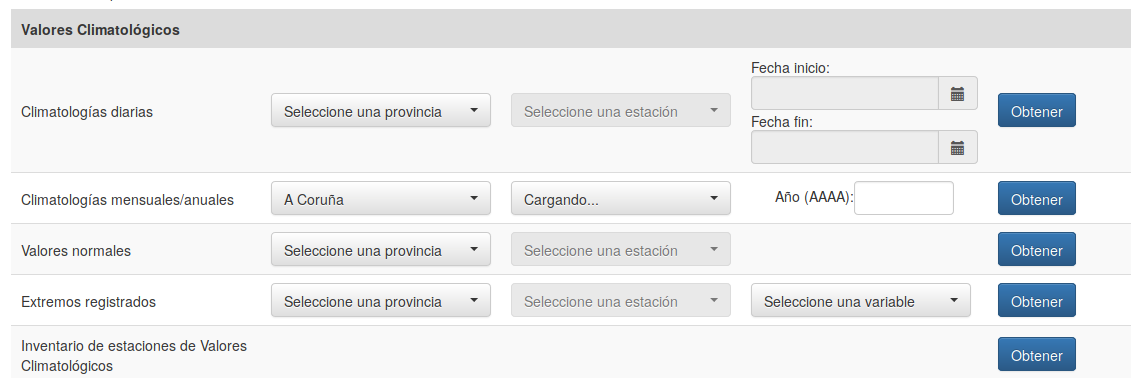
\includegraphics[width=\textwidth]{panel_aemet}
\end{figure}

Una vez descargados, hemos obtenido para cada ciudad un JSON como el siguiente:

\inputminted{json}{apendices/datos_aemet.json}

\section{Procesado}

Para cada mes, para cada archivo, se extrae el parámetro \verb|tm_mes| (que indica la temperatura media del mes) y se genera un documento CSV para poder tratarlo mejor:

\begin{lstlisting}
ft,2012,1,10.6
...
cg,2018,12,14.2
\end{lstlisting}